\documentclass[twocolumn]{article}
\usepackage{graphicx,amsmath}
\graphicspath{{figures/}{./}}
\newcommand{\roi}{frontal}
\title{A Test Paper on Connectivity}
\author{Author One \and Author Two}
\begin{document}
\maketitle
\begin{abstract}
We tested 40 participants and found that \roi{} connectivity decreased ($t = -2.10$, $p = 0.041$).
\end{abstract}
\section{Introduction}
\label{sec:intro}
Stimulation changes connectivity \cite{smith2020}. Respiration matters too \cite{lee2021}. As shown in Figure~\ref{fig:one} and Table~\ref{tab:one}, the effect is robust.
The model is $y_{ij} = \beta_0 + \beta_1 t_{ij} + u_i + \epsilon_{ij}$ with random intercepts.
\section{Methods}
\subsection{Participants}
Forty-two participants were recruited from the clinic. Each completed six scanning sessions over five days of treatment.
\begin{equation}
r = \frac{\sum (x - \bar x)(y - \bar y)}{\sqrt{\sum (x-\bar x)^2 \sum (y - \bar y)^2}}
\label{eq:r}
\end{equation}
\begin{figure}[t]
\centering
\includegraphics[width=\columnwidth]{fig1}
\caption{Connectivity by day. A) Active arm. B) Sham arm.}
\label{fig:one}
\end{figure}
\begin{table}[t]
\caption{Participant characteristics.}
\label{tab:one}
\centering
\begin{tabular}{lrr}
\hline
Group & N & Age \\
\hline
Active & 21 & 42.1 \\
Sham & 19 & 44.3 \\
\hline
\end{tabular}
\end{table}
\section{Results}
Connectivity decreased by 0.010 per day in the active arm (Section~\ref{sec:intro}).
\begin{figure*}[t]
\centering
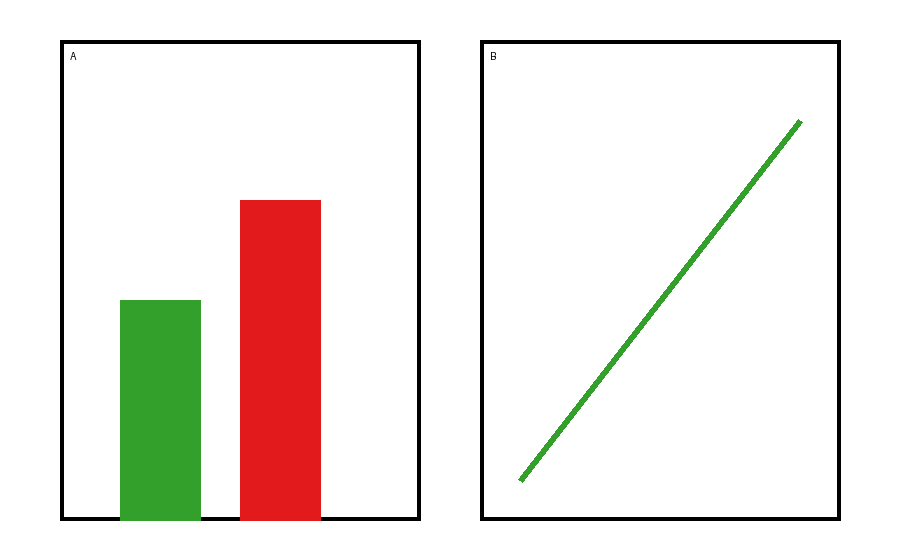
\includegraphics[width=0.45\textwidth]{fig2.png}
\includegraphics[width=0.45\textwidth]{figures/fig1.png}
\caption{Two subfigures side by side.}
\label{fig:two}
\end{figure*}
\section{Discussion}
Effects were modest.
\bibliographystyle{plain}
\bibliography{refs}
\end{document}
